\documentclass[12pt]{report}
\usepackage{hyperref}
\usepackage{fancyhdr}
\usepackage{tcolorbox} % Read the docs for this to see how to make fancy boxes
\usepackage{amsmath}
\usepackage[style=ou]{biblatex}
\renewbibmacro{in:}{}
\usepackage{inputenc}
\usepackage{tabularx}
\usepackage{array}
\usepackage[style=british]{csquotes}

\title{\LARGE Hubble Tension: Constraining the Hubble parameter using time-delay gravitational lensing experiments and comparison with other methods %

}
\vspace{1cm}
\author{Lauren Jade Thomas}
\date{\today}


% Configuration of headings
%\pagestyle{fancy}
%\fancyhf{} % Get rid of default headers and footers
%\rhead{\chapterautorefname}
%\lhead{Back and to the left}
%\rfoot{My foot hurts.}
%\lfoot{Page \thepage}
%\cfoot{I'm very centered}
%\chead{Place forehead here}

% Citation config
\addbibresource{bibliography.bib}

\makeatletter
\renewenvironment{titlepage}
 {%
  \if@twocolumn
    \@restonecoltrue\onecolumn
  \else
    \@restonecolfalse\newpage
  \fi
  \thispagestyle{empty}%
 }
 {%
  \if@restonecol
    \twocolumn
  \else
    \newpage
  \fi
 }
\makeatother

\begin{document}
%\let\thesection=1
\addcontentsline{toc}{chapter}{Title Page}
\maketitle

\setlength{\parskip}{5pt}

\setlength{\parindent}{0pt} 
%\titleformat{\chapter\normalfont\large}

\renewcommand{\theequation}{\arabic{equation}}


\addcontentsline{toc}{chapter}{Abstract}
\begin{abstract}
Hubble tension is one of the biggest mysteries facing modern observational cosmologists' in recent years. For nearly 100 years, researchers and theorists alike have been trying to calculate the rate at which the universe is expanding. Our current understanding of the universe is dependent on the $\Lambda$CDM model; however, when this model is used in conjunction with early universe probes, a statistically significant $4\sigma$ to $6\sigma$ discrepancy appears when compared to multiple, model-independent, late universe probes that utilise measured distances and observed redshifts. In this review, I primarily focus on one such late universe technique; strong gravitational lensing. I start by outlining the underlying theory of the phenomenon with a brief mathematical framework, including an introduction to how galaxy lenses are modelled and how these systems are used to calculate the Hubble constant. I provide a brief overview of both early and late universe probes and the most current results determined by these methods, focusing on recent strong gravitational lensing surveys and their model designs. I look at how we could reconcile this tension, whether it can be explained by invoking systematic uncertainties or whether refinements in lens modelling approaches, future data collection and processing techniques  (or a combination of all three) will be sufficient for eliminating this tension with strong gravitational lensing alone or if there is a call to re-evaluate our current cosmological model. 
\end{abstract}

\addcontentsline{toc}{chapter}{Table of contents}
\tableofcontents

\chapter{Introduction}

\section{Background}

The Hubble constant is the rate at which the universe expands at any given time. The Hubble constant is derived from Hubble's law, the observation in physical cosmology that galaxies are moving away from the Earth at speeds that are proportional to their distance. It is one of the most compelling pieces of evidence that supports Big Bang Cosmology, which underpins our present-day understanding of the universe.

The Hubble constant, $H_0$, can be calculated from astronomical data in multiple ways. In this review, I focus on using strong gravitational lensing systems. \textcite{Refsdal1964} concluded that per the laws of General Relativity, the path of light from a background star would be deflected by the gravitational field of a foreground star. This phenomenon has been well tested, and we have even observed the gravitational lensing by entire galaxies (and galaxy clusters) since the discovery of the first gravitationally lensed quasar by \textcite{Walsh1980}. Since then, this technique has been used extensively to constrain the value of the Hubble constant.

In this project, I examine how this technique has been used to calculate values of the Hubble constant. Explore why different lensing systems and early and late universe methods do not always return the same value; after all, the Hubble constant should be constant.

\section{Objectives}

\begin{enumerate}
    \item Survey and summarily describe the underlying theory behind the various approaches for calculating the Hubble constant.
    \item Explain how strong gravitational lensing can be and is used to calculate the Hubble constant to a high degree of precision and how this is achieved. 
    \item Explore recent experimental work that uses time-delay cosmography to calculate the Hubble constant, evaluating the underlying methodology's strengths and weaknesses and how different techniques lead to differing values for $H_{0}$.
    \item Suggest how the discrepancy between early and late values of $H_{0}$ could be resolved in future, examining sources of error and potential gaps in our understanding. 
\end{enumerate}

\section{Scope of work}

This project focuses on gravitational time delay lensing, how this technique is used in the field of time delay cosmography to calculate the universe's rate of expansion, and how these values conflict with those derived using direct and indirect methods. The underlying theory of other methods will not be discussed in great detail, but an overview will be provided where necessary for comparison purposes.

\section{Search methodology}

\begin{itemize}

    \item A combination of SAO/NASA astrophysics data system, \textcite{ADS2022}, arxiv.org, and google scholar primarily searching for "Gravitational lensing" AND "Hubble tension" (or AND "Hubble constant") and references therein.
    \item Reviewing the publications from large research collaborations websites (notably \textcite{TDCOSMO} \& \textcite{H0LiCOW} and papers referenced therein).
    \item Evaluated each paper using the PROMPT criteria, \textcite{OU2014}, to evaluate the suitability of papers selected to shortlist for the report's central themes.
    \item The papers and books included in the resources provided as part of the SXP390 module materials included in the gravitational lensing topic: primarily a citation search from the 33rd Saas-Fee Advanced Course - Gravitational lensing: Strong, Weak \& Micro, \textcite{Kochanek2004}.
\end{itemize}


\chapter{Gravitational lensing theory}

\vspace{-0.75cm}

\section{General Relativity to Gravitational lensing}

The main takeaway of the theory of General Relativity is that the presence of any mass alters the geometry of spacetime; it is because of this fundamental property of spacetime that gravitational lensing occurs. Photons emitted from astronomical sources are assumed to be radiated uniformly in all directions; when we think of light as a particle, we expect the light to travel in a straight line between source and observer. Light would travel in straight lines if spacetime were entirely flat; it is not at local scales.

This review focuses specifically on strong gravitational lensing; strong lensing occurs when a lens has a mass density in projection above a particular critical density (as defined by the individual system) which leads to both the multiplication and magnification of the source, as seen by the observer. In simple terms, it can be understood as an optical mapping between the (true) source plane and an observed image plane. However, gravitational lenses differ from conventional optical lenses because they have no single focal point but rather lines of theoretically infinite magnification known as critical lines. When these critical lines are transferred back to the source plane, they are called caustics. The location of these lines is both dependent on the relative distance between the source and lens plane and the matter distribution within
the lens itself. The position of the source with respect to its relevant caustic (as governed by its distance from the lens) determines the arrangement of the (often multiple, discrete) images and their magnifications.

\subsection{Deflection angle}

\begin{figure} [h]
    \centering
    \includegraphics[width = 0.75\textwidth, height = 5.5cm]{pmlens.jpeg}
    \caption{Simple point mass lens diagram, where S is the position of the source, O is the position of the observer, M is the mass of the lens, and $\xi$ is the impact parameter—created by author.}
    \label{fig:figure1}
\end{figure}


Suppose we examine a point mass gravitational lens (Figure 2.1) and the equations that govern General relativity (for a complete derivation, see \textcite{Carroll2004}) we can derive an equation that tells us the gravitational deflection angle $\hat{\alpha}$ in terms of the mass of the lens, M, the Gravitational constant, G = $6.6743 \times 10^{-11} \ m^{3} \ kg^{-1} \ s^{-2}$ and impact parameter $\xi$.  

\begin{equation*}
    \hat{\alpha} = \dfrac{4GM}{\xi}
\end{equation*}

\subsection{Thin screen approximation}

Most of the deflection by a gravitational lens occurs near the lens, within $z \sim \xi$. This allows us to treat all deflection as if it occurs in the lens plane. We can use the thin screen approximation because the distance between the lens and source and the lens and observer is far more significant than the lens size.

\newpage

\subsection{The Lens equation}

\begin{figure}[h]
    \centering
    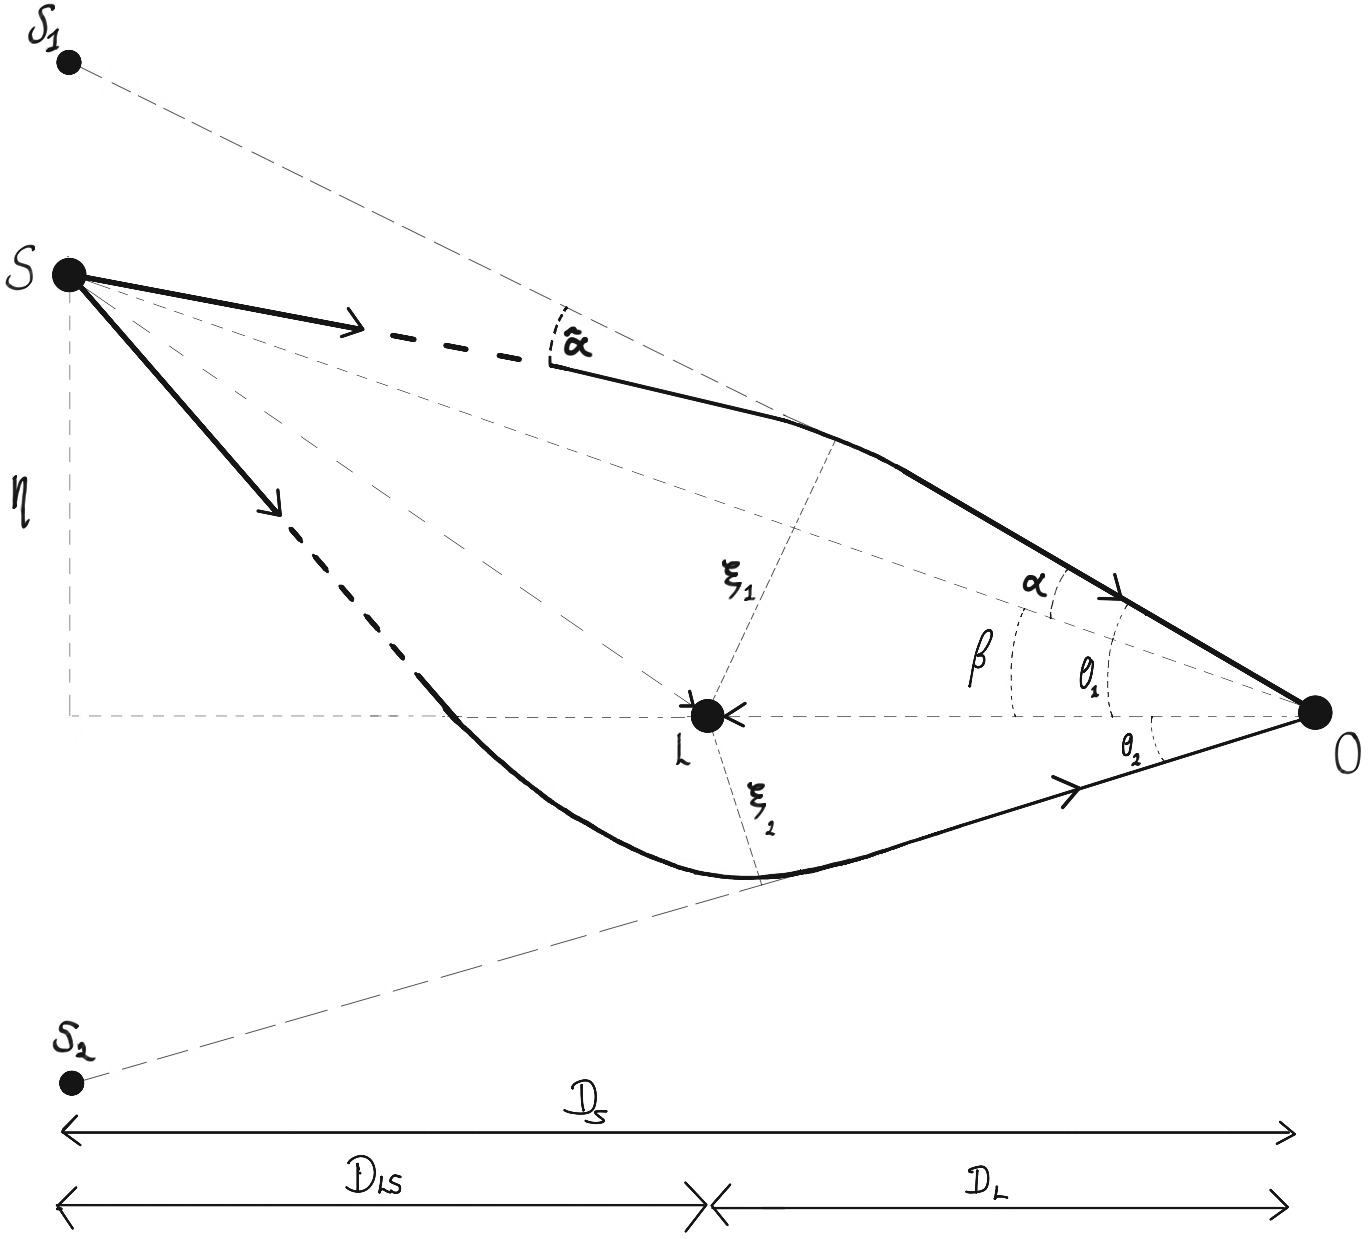
\includegraphics[width =0.8\textwidth, height = 8.5cm]{figure_1.jpeg}
    \caption{A Strong gravitational lensing system wherein S, L and O are the source, lens and observer, respectively. $\hat{\alpha}$ is the deflection angle, $\alpha$ is the scaled deflection angle, $\eta$ is the 2D position of the source in the source plane, $\beta$ is the angular position of the source (if there were no lens), and $\theta$ is the observed angular position. $\xi_{1}$ and $\xi_{2}$ are the impact parameters for the top and bottom paths, respectively. Created by author.}
    \label{fig:Figure2}
\end{figure}


If we apply the thin screen approximation to the strong gravitational lensing system outlined in Figure 2.2, the small-angle approximation can be used; as well as the thin lens equation:

\begin{align*}
    \alpha(\theta) &= \dfrac{D_{LS}}{D_{S}} \ \hat{\alpha}(D_{S}\theta) & \eta &= D_{S} \ \beta \\
    \beta &= \theta - \alpha(\theta) & \xi &= D_{L} \ \theta
\end{align*}

\newpage


In our understanding of the universe, the $\Lambda$CDM model specifies that the universe is flat. These equations hold true as long as space has zero curvature; if space has any degree of curvature, then $D_{LS} \neq D_{S} - D_{L}$. This means that gravitational lensing is one of the few model-independent tests on whether this assumption is accurate. 

The extent of a mass's lensing effect can be determined mathematically; in the case of a point mass, it would have a perfectly circular lens with a radius equal to the lens's Einstein radius, $\theta_{E}$. 

\begin{equation*}
    \theta_{E} = \sqrt{\dfrac{4GM}{c^{2}} \dfrac{D_{LS}}{D_{S}D_{L}}}
\end{equation*}

When $\beta > \theta_{E}$, the source is weakly lensed, which results in one weakly distorted image. When $\beta < \theta_{E}$, the source is strongly lensed, and multiple images are formed. If $\beta = \theta_{E}$ then an Einstein ring is formed. As in Figure 2.2, in strong gravitational lensing systems, there can be multiple solutions/values for $\beta$ and, thus, multiple discrete images. For strong lensing to occur; the projected surface density, $\Sigma$, must also exceed the critical density given by

\begin{equation*}
    \Sigma_{CR} = \dfrac{c^{2}}{4\pi G} \ \dfrac{D_{S}}{D_{L}D_{LS}}
\end{equation*}

\subsection{Magnification}

Gravitational lensing preserves surface brightness but alters the apparent solid angle of the source due to magnification. In the general case, magnification calculated using the lens equation is

\begin{equation*}
    \mu = \Bigg| \ det \bigg( \dfrac{\partial \beta}{\partial \theta} \bigg) \ \Bigg|^{-1} \equiv \Bigg| \ det \bigg( \dfrac{\partial \beta_{i}}{\partial \theta_{j}} \bigg) \ \Bigg|^{-1}
\end{equation*}

If the lens is circularly symmetric, this reduces to 

\begin{equation*}
    \mu = \dfrac{\theta}{\beta} \dfrac{\partial \theta}{\partial \beta}
\end{equation*}

\newpage

\textbf{In the example of a point mass: }

Images occur at 

\begin{equation*}
    \theta_{\pm} = \frac{1}{2} \ ( \beta \pm \sqrt{\beta + 4\theta_{E}^{2}}), \ \ u = \beta \theta_{E}^{-1}
\end{equation*}


Magnification is 

\begin{equation*}
    \mu_{\pm} = \Bigg[1 - \bigg(\dfrac{\theta_{E}}{\theta_{\pm}} \bigg)^{4} \Bigg]^{-1} = \dfrac{u^{2} +2}{2u\sqrt{u^{2} +4}} + \frac{1}{2}
\end{equation*}

If the value is positive, the source is magnified. If it is negative, it can go either way; it is dependent on the system.

The total magnification is 

\begin{equation*}
    \mu = |\mu{+}| + |\mu_{-}| = \dfrac{u^{2} +2}{u\sqrt{u^{2} +4}}
\end{equation*}

When the source is on the Einstein ring: $\beta = \theta_{E}, u = 1$


\subsection{Shapiro Time Delay}

Due to the presence of the mass-created lens, light rays take different paths toward the observer and therefore take different amounts of time to reach the observer. The time delay between each image (as measured by the total redshift of each image) underpins how time-delay cosmography can experimentally determine the Hubble constant. Time-delay measurements have the additional benefit of being completely independent of the cosmic distance ladder. 

\newpage

Time delays were first outlined by \textcite{Shapiro1964} and are defined by the equation:
 
\begin{equation*}
    \Delta t = - \int \Phi \ ds
\end{equation*}

The total time delay is the sum of the path lengths from deflection and the gravitational time delay. 

\begin{equation*}
    \begin{split}
    t(\Vec{\theta}) &= \dfrac{(1 + z_{d})}{c} \dfrac{D_{L}D_{S}}{D_{LS}} \Bigg[ \frac{1}{2} (\Vec{\theta} - \Vec{\beta})^{2} - \psi(\Vec{\theta}) \Bigg] \\
    &= t_{geom} + t_{grav}
    \end{split}
\end{equation*}

\section{Galaxy Lensing and Constraining $H_{0}$}

\subsection{Single Isothermic Sphere}

Galaxy lenses require that we accurately account for the distribution of matter within the lens. The simplest way to do this is by assuming a model that treats all the galactic mass like particles in an ideal gas. Therefore we can use the ideal gas equation and related phenomena to define the system. This approach allows lenses created by a galaxy (or a cluster of galaxies) to be treated like a point-mass lens. As such, we expect a minimum of two images to be formed. The magnification can be substantial, especially for sources directly aligned with the lens; when this happens, an Einstein ring is formed. 

\subsection{Mass Determination}

The time-delay depends on the total matter distribution within a lensing galaxy, both baryonic and dark. A simple estimate of the total mass can be obtained if we assume a perfectly spherical lens because the critical mean density will equal the mean surface density contained within the Einstein radius. 

\vspace{10mm}

In practice, one needs to take into account the mass-sheet transformation (MST); the mass distribution, $k(\theta)$, isotropically scales with $\lambda$ (term representing the MST). (\textcite{Falco1985})

\begin{equation*}
    \kappa_{\lambda}(\theta) = \lambda \kappa(\theta) + (1 - \lambda)
\end{equation*}

The MST scales everything from the source position to $H_{0}$ and time-delay distance equally, and it is impossible to determine from optical images alone - this is called mass-sheet degeneracy (MSD) (\textcite{Schneider2013}). However, including spectroscopy or stellar kinematics data can break this degeneracy; it is also worth considering that the MST also has external components; for example, the distribution of matter in the line-of-sight (LOS) should also be accounted for - \textcite{Rusu2017}.

Whilst the time-delay distance is most sensitive to the value of $H_{0}$; it is still weakly dependent on the values of the matter density, $\sigma_{m}$, dark energy density, $\sigma_{de}$, the dark energy equation of state, $w$, and the curvature parameter, $\sigma_{k}$. (\textcite{Suyu2010} \& \textcite{Linder2011}).


\subsection{$H_{0}$ Determination}

As outlined above, the total time-delay has two components; geometric and gravitational. The geometric element can be found from the angular distances $D_{L}$, $D_{S}$ and $D_{LS}$ and the redshift, z. The gravitational component $\phi(\theta, \beta)$ is dependent on the mass distribution (convergence) $\kappa(\theta)$ since $\kappa(\theta) = \frac{1}{2}\nabla^{2}\psi({\theta})$ where $\psi({\theta})$ is the lensing potential of the galaxy. This is why lens modelling is crucial because, without it, there is no way to account for the MST's scaling of $H_{0}$. Time-delay can be measured, so time-delay distance $D_{\Delta t}$ can be calculated. The Hubble constant is inversely proportional to the scales of the universe, ergo $H_{0} \propto D_{\Delta t}^{-1}$. The degeneracy needs to be broken to calculate a value for $\lambda$, so an accurate inference of $H_{0}$ can be made.

\chapter{Constraining $H_{0}$ experimentally}

\vspace{-0.75cm}

Methods for determining the Hubble constant from experimental data fall into two distinct groups; indirect and direct. The currently accepted values of the cosmological parameters (Table 3.1) are derived from indirect methods. These methods utilise the analysis of the anisotropies in Cosmic Microwave Background Radiation (CMBR). These are called early universe measurements in the literature since they look at matter distribution 'shortly' after the big bang. Direct methods, or late universe measurements, pertain to calculations made from astronomical phenomena researchers have directly observed. 

\section{Early Universe Probes}

\subsection{WMAP and Planck}

Efforts to calculate the value of the Hubble constant in the early universe utilise the anisotropies in the CMBR. Using the data gathered by both the Wilkinson Microwave Anisotropy Probe (WMAP) and the European Space Agency's (ESA) Planck probe (also known as the Planck Collaboration), detailed images of the CMBR were created.

\newpage

\begin{figure} [t]
    \centering
    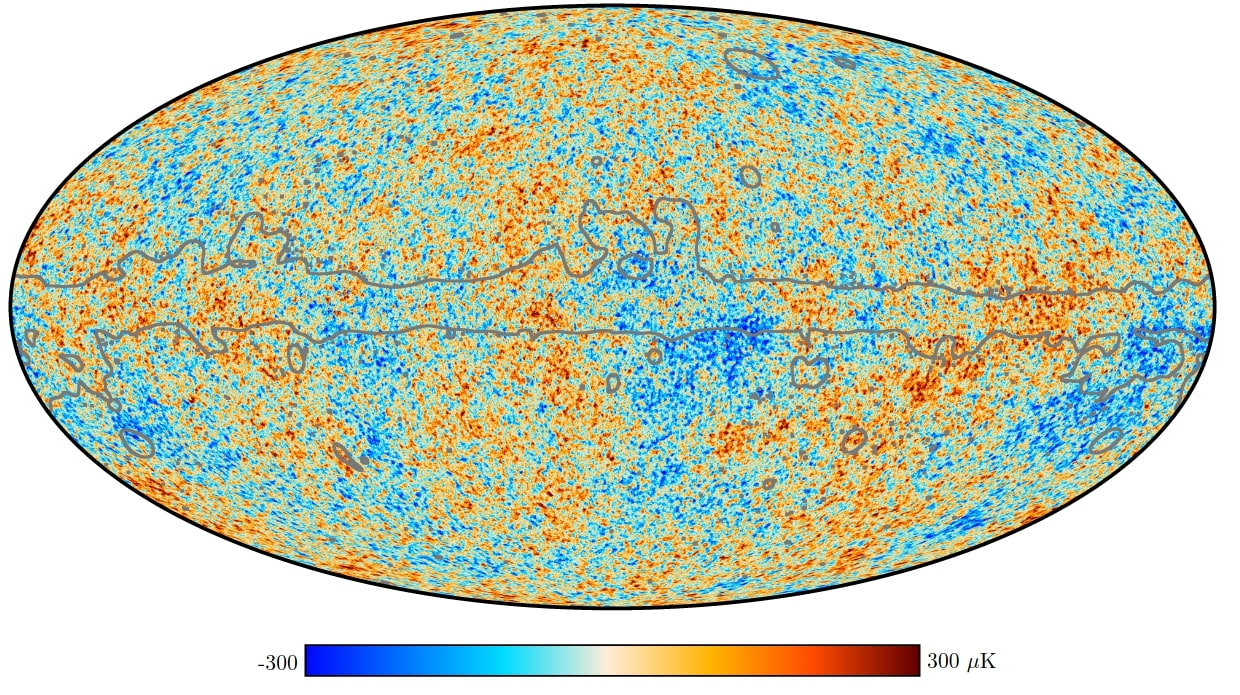
\includegraphics[width = 0.75\textwidth, height = 5.5cm]{figure3.jpg}
    \caption{The 2018 Planck map shows the temperature anisotropies found in the CMB. The bright yellow and red spots represent areas of increased temperature, which directly correspond to matter distribution in the early (and present-day) universe. (\textcite{ESA2018}).}
    \label{fig:figure3}
\end{figure}

\setlength{\arrayrulewidth}{0.2mm} %border thickness

\setlength{\tabcolsep}{8pt} %space between text and border

\renewcommand{\arraystretch}{1.1} %changes row height

\begin{table}[h!]
    \centering
    \begin{tabular}{|c|c|c|}
\hline
        \textbf{Parameter:} & \textbf{Symbol:} & \textbf{Final Value:}\\
\hline
\hline
        Scalar spectral index & $n_{s}$ & $0.9665 \pm 0.0038$ \\
\hline
        Age of the universe & $t_{0}$ & $13.787 \pm 0.020 \ \times 10^{9}$ years \\
\hline
        Optical depth due to reionization & $\tau$ & $0.0561 \pm 0.0071$ \\
\hline
        Physical baryon density & $\Omega_{b}h^{2}$ & $0.02242 \pm 0.00014$ \\
\hline 
        Physical dark matter density & $\Omega_{c}h^{2}$ & $0.11933 \pm 0.0041$ \\
\hline
        Curvature fluctuation $\text{amplitude}^{[1]}$ & $\Delta^{2}_{R}$ & $2.441^{+0.088}_{-0.092} \times 10^{-9}$\\ 
\hline
        Hubble constant $(km \ s^{-1}Mpc^{-1})$ & $H_{0}$ & $67.66 \pm 0.42$ \\
\hline
        Dark energy density & $\Omega_{\Lambda}$ & $0.6889 \pm 0.0056$ \\
\hline
        Matter density & $\Omega_{M}$ & $0.3111 \pm 0.0056 $ \\
\hline
    \end{tabular}
    \caption{The six independent parameters of the $\Lambda$CDM model of the universe and the calculated values of the Hubble constant, Dark Energy density and overall matter density from \textcite{Aghanim2020}. [1] - From \textcite{Jarosik2011}} 
    \label{tab:my_label}
\end{table}

\subsection{Baryonic Acoustic Oscillations (BAOs) and BOSS}

The anisotropies visible in the CMBR are directly related to the position of matter in the present-day universe. The physics of propagation of baryonic matter before recombination is well understood, which allows cosmologists to calculate the size of the sound horizon at recombination. The distribution of matter in the CMBR and the present-day universe is the same; as the universe has aged, it has expanded at the rate defined by the Hubble constant equally in all directions. By comparing the position of galaxy clusters (for example) to the anisotropies in the CMBR, researchers can calculate the expansion rate without relying on data from other techniques, \textcite{Eisenstein2005}.

The latest result derived using this technique is from \textcite{Alam2021}, the team behind the extended Baryonic Oscillations Spectroscopic Survey (eBOSS) found using data from the Sloan Digital Sky Survey's 16th data release (SDSS DR16) that $H_{0} = 68.20 \pm 0.81 \ km \ s^{-1} Mpc^{-1}$ at a 68\% confidence level (CL) when assuming the standard $\Lambda$CDM model. 

\subsection{Dark Energy Survey}

The Dark Energy Survey (DES) employed the 'inverse distance ladder' method to calibrate the absolute magnitude of 329 Type Ia Supernovae (SNIa), using absolute distance measurements derived from BAOs. \textcite{MacAulay2019} found that when used in combination, the value of $H_{0} = 67.8 \pm 1.3 \ km \ s^{-1} Mpc^{-1}$ (68\% CL) when taking into account statistical and systematic uncertainties. This value agrees with values calculated from the CMBR and negates the previous tension. 

\newpage

\section{Late Universe Probes}

\subsection{Cosmic Distance Ladder}

Direct measurements that allow the calculation $H_{0}$ are many and varied. One of the most common techniques relies on the cosmic distance ladder, which allows astronomers to calculate astronomical distances through various methods. The Hubble constant can be calculated when the distance to an object with known composition and redshift is examined. The use of trigonometric parallaxes is limited to objects within approximately 1000 parsecs of Earth, so standard candles are used. A standard candle is an object of known luminosity; by comparing the known luminosity to the observed brightness, the distance can be modelled using an inverse-square law.  

This technique has been used to calculate various values of $H_{0}$; the Supernovae $H_{0}$ for the Equation of State (SH0ES) team recently presented their findings from a 15-year effort to create a robustly calibrated distance ladder. By using the distances to hundreds of Cepheid variable stars and SNIa to calibrate their distance ladder they generated an estimate of $H_{0} = 74.03 \pm 1.42 \ km \ s^{-1} Mpc^{-1} $ (\textcite{Riess2019}).

The distance ladder is reliant on calibration; the Carnegie-Chicago Hubble Program (CCHP) used stars at the Tip of the Red Giant Branch (TRGB) to calibrate their distance ladder and found $H_{0} = 69.8 \pm 0.6 \ \text{(statistical)} \pm 1.6 \ \text{(systematic)} \ km \ s^{-1} Mpc^{-1}$. These results from \textcite{Freedman2021} significantly reduce the tension between early and late universe measurements but rely on local measurements and appear to diverge at larger distances. The most recent paper from SH0ES, \textcite{Riess2022}, uses both Cepheid and TRGB calibration of SNIa and found $H_{0} = 72.53 \pm 0.99 \ km \ s^{-1} \ Mpc^{-1}$, so whilst accuracy appears to be increasing, we cannot wholly disregard the need to improve either our methods or understanding.

\newpage

\subsection{Strong Gravitational Lensing}

\vspace{-0.5cm}

\begin{figure} [ht!]
    \centering
    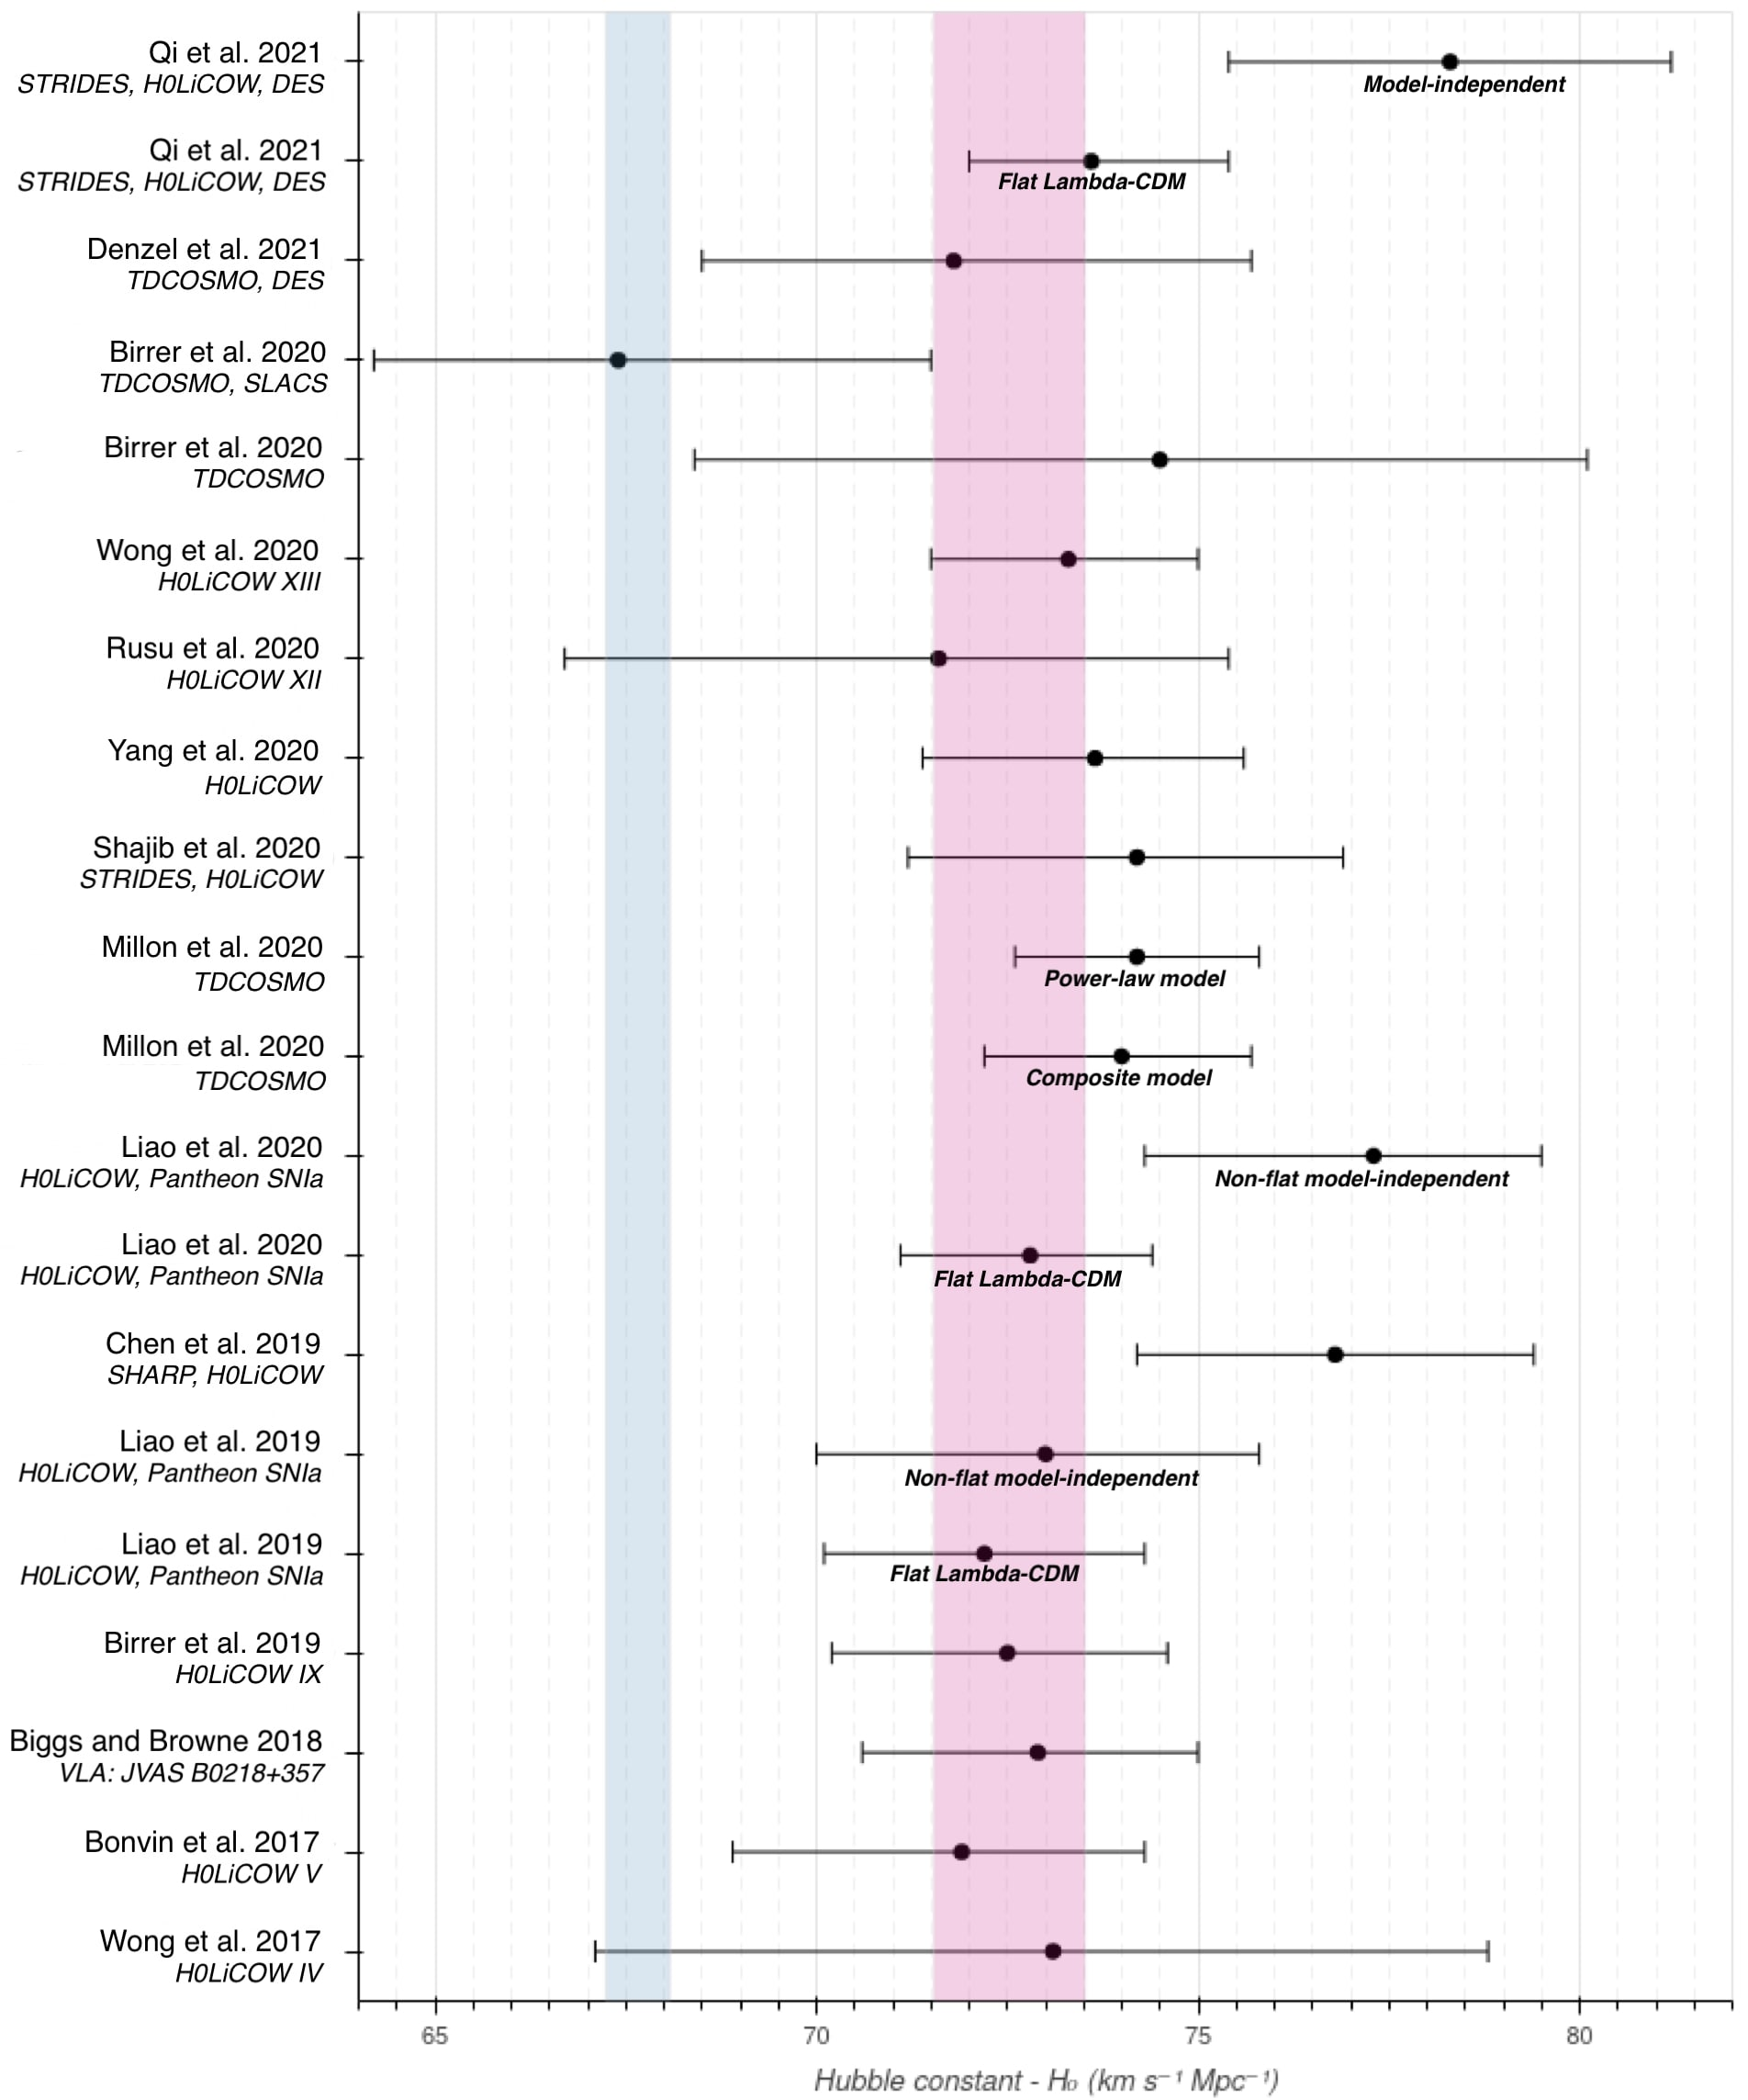
\includegraphics[width = \textwidth, height = 15cm]{figure4.jpg}
    \caption{A whisker plot of strong gravitational lensing derived values of the Hubble constant from 2017 to 2022. Different analyses from the same paper are listed separately. The blue band represents the values from Planck, \textcite{Aghanim2020} and the pink band the most recent results from SH0ES, \textcite{Riess2022} - Created by author.}
    \label{fig:figure4}
\end{figure}


Unfortunately, these values exist in significant tension with early universe measurements. The main challenge is to create an accurate mass distribution model which can be used to make an accurate inference of the time-delay distance. 

Lens mass distribution models are parameterised mass models where observational data define the parameters. However, it is possible to create a model that perfectly fits the observed characteristics of a lensing system, leading to a completely wrong inference of the time-delay distance (\textcite{Bonvin2017}). One needs to take special care when attempting to break the Mass-Sheet degeneracy; the use of a simple power-law density model can lead to a bias on $H_{0}$ of between 20-50\% (\textcite{Xu2016}). This can, however, be mitigated with the use of stellar kinematics data, \textcite{Sonnenfeld2018} found that the combination of the power-law density profile and stellar kinematics data for double-lensed systems can be used to calculate $H_{0}$ with a 3\% accuracy.

It is worth highlighting that \textcite{Birrer2019} modelled the doubly imaged quasar SDSS 1206+4332 using a composite model for the deflector galaxy, taking into account both baryonic and dark matter and the deflector galaxy's velocity dispersion. Combined with the characteristics of the quasar host galaxy, nearby perturbing galaxies and the line of sight structure, $H_{0} = 68.8^{+5.4}_{-5.1}  \ km \ s^{-1} Mpc^{-1}$ with an overall precision from a single lens of 7.2\%. However, when combined with three previous H0LiCOW lenses, taking into account the statistical likelihood of these systems, they found $H_{0} = 72.5^{+2.1}_{-2.3} \ km \ s^{-1} Mpc^{-1}$. Whilst the uncertainties are significant, this value does appear to be in relative agreement with early universe measurements.

It, therefore, becomes clear that values calculated from strong gravitational lenses are only ever as precise as their lensing models. Numerous components must be considered, as discussed above and in Chapter 2; it can be challenging to constrain all the possible compounding variables with the data available. Therefore researchers have started to use external datasets to help 'fill in the gaps' as outlined below. 

\newpage

\subsection{Combining Multiple Datasets}

The measurements from multiple lensing systems are often combined to form a composite sample, and lenses are also frequently reanalysed. For example, \textcite{Yang2020} reanalysed four of H0LiCOW's (H0 Lenses in COsmograil's Wellspring) lenses, for which they had calculated time-delay distances and distances inferred from stellar kinematics data and found $H_{0} = 73.65^{+1.95}_{-2.26} \ km \ s^{-1} Mpc^{-1}$. TDCOSMO I, (\textcite{Millon2020}) combined six lenses from the H0LiCOW sample and one lens from STRIDES (STRong lensing insights into Dark Energy Survey) and when assuming a power-law lens models, calculated $H_{0} = 74.2 \pm 1.6 \ km \ s^{-1} Mpc^{-1}$. 

TDCOSMO IV (\textcite{Birrer2020}) reanalysed the TDCOSMO dataset, eschewing previous mass models and choosing to constrain models using only stellar kinematics data and found $H_{0} = 74.5^{+5.6}_{-6.1} \ km \ s^{-1} Mpc^{-1}$. Combined with imaging and spectroscopy data from 33 strong lenses in the Sloan Lens ACS (SLACS) dataset and joint hierarchical analysis, they calculated $H_{0} = 67.4^{+4.1}_{-3.2} \ km \ s^{-1} Mpc^{-1}$. 

The findings from this analysis do not statistically invalidate the mass models used in the previous H0LiCOW analyses; it does highlight the need for a thorough understanding of the mass profiles of elliptical deflector galaxies. This finding is an excellent example of the potential of using external datasets to create a generalised statistical model. However, the errors are significant, partially due to the uncertainties in the stellar kinematics data. In part due to the use of spherical jeans modelling (model of the stellar velocity dispersion) as well as the 10\% scatter in the values of $\lambda_{int}$ used to break the MSD of the TDCOSMO lenses and partially due to the assumption that the lenses are from the same parent population and therefore share significant characteristics. 

In the future, they expect that with additional time-delay and non-time-delay lenses from SLACS and the Strong Lensing Legacy Survey, precision will increase to 1.2\%, thereby resolving the Hubble tension at $3\sigma$ to $5\sigma$ without making assumptions about the radial mass profiles of deflector galaxies, \textcite{Birrer2021}. 

The values presented thus far all rely on the current understanding of the universe, the flat $\Lambda$CDM model. Some attempts to separate the calculation of $H_{0}$ from the late behaviour of the $\Lambda$CDM model have been undertaken, \textcite{Liao2019} use four strongly lensed quasar systems from H0LiCOW and data from the Pantheon SNIa compilation, using a gaussian process regression to create an estimate of $H_{0} = 72.2 \pm 2.1 \ km s^{-1} Mpc^{-1}$ in a flat universe, ($H_{0} = 73.0^{+2.8}_{-3.0} \ km \ s^{-1} Mpc^{-1}$ when allowing for a cosmic curvature density $\sigma_{k} = [-0.2, 0.2])$, later updated in \textcite{Liao2020} with the use of six lenses from H0LiCOW to $H_{0} = 72.8^{+2.1}_{-1.7} \ km s^{-1} Mpc^{-1}$ and $H_{0} = 77.3^{+2.2}_{-3.0} \ km \ s^{-1} Mpc^{-1}$ in a similarly non-flat universe.


\chapter{Reconciling Early and Late Measurements}

\vspace{-0.75cm}

How can we reconcile these results with each other, and is it possible to resolve this tension with our current understanding? 

The measurement of CMB anisotropies has resulted in incredibly precise values of the six required independent cosmological parameters of the standard model of Big Bang cosmology. (In this case, Occam's razor requires a minimum of six independent parameters to create an acceptable fit for current observations). If we assume that the current model is correct, the calculated value of the Hubble constant from this data set ought to be the actual value. As I have shown so far, an overwhelming body of evidence from direct observations contradicts this value.

\section{Systematic Errors}

The most cynical explanation is to focus on these methods' often significant uncertainties; however, this feels very reductionist. Any single systematic error would need to affect every calculated value equally. A singular systematic error is improbable, if not impossible, given the size of the discrepancy between calculated values from indirect and direct methods and the sheer number of independent direct methods yielding similar values. Each method is independent of the others and individually affected by different systematic uncertainties, yet all agree. The likelihood of completely independent systematic errors affecting each experiment in all these measurements, in the same way, feels slim to none. However, the systematic errors in CMB measurements cannot explain this tension either. 

There is a formal way to combine unknown systematic errors between multiple experiments using the BACCUS (BAyesian Conservative Constraints and Unknown Systematics) framework. This method was first introduced by \textcite{Bernal2018} to allow for combining multiple direct methods, all of which are independent of each other. Their average included direct measurements using the distance ladder, BAOs, time-delay cosmography, cosmic clocks (the use of differential ages of old elliptical galaxies that estimate of the inverse of the Hubble parameter $H(z)^{-1}$) and light curve analysis from SNIa. They found a total average of $H_{0} = 72.7 \pm 1.2(2.9) \ km \ s^{–1} Mpc^{–1}$ at a confidence level of 68(95)\%, which is still in significant tension with the value calculated by Planck. 
 

\section{Future Research}

The question becomes; why is there such a significant difference? It can't be denied that there is room for improvement in lens modelling methods; there is an obvious need for more constraints on these mass models. At the time of writing, the first images from the James Web Space Telescope/Near InfraRed Camera (JWST/NIRCam) have recently become available. \textcite{Caminha2022} [preprint: July 2022] have just unveiled the first strong gravitational lens mass model created using this new data. They generated a mass model for the lens SMACS J0723.3-7327 from pre-JWST data (19 multiple images from 6 background sources, 4 of which have associated spectroscopic data) and a refined model from JWST data (an additional 27 images and no additional spectroscopic data). The uncertainties in the JWST model are already 33\% lower without the inclusion of spectroscopic data. With the inclusion of the spectroscopic data included in \textcite{Mahler2022} [preprint: July 2022], the mass model of SMACS J0723.3-7327 will undoubtedly become even more precise. Only time will tell if this increase in precision modelling will resolve the Hubble tension or if our current cosmological model needs to be adapted. 

So far, our attempts to tackle the problem of the Hubble tension all rely on one thing; data. With surveys from the JWST and the Rubin Observatory Legacy Survey of Space and Time (LSST) Dark Energy Science Collaboration (DESC), we are anxiously awaiting an explosion in the amount of data available. This, however, poses its problems. Converting these data points into a workable model for each lens is time-consuming and laborious.

I find the approach suggested by \textcite{Sonnenfeld2021} and \textcite{Sonnenfeld2022} to be the most hopeful for breaking the $H_{0}$ lens model degeneracy with observational data alone. However, he determined that the sample size required to create a parameterised model for a population of galaxies would require the computer modelling of well over 100 lenses supplemented by data from non-lensing galaxies - a population of solely strongly lensing galaxies is inherently biased - to determine the true properties of a galaxy population. Creating 100 models from real observational data has been unachievable thus far, even if we had data on 100 lenses.

It is a genuine possibility that we will be able to collect enough data to break the degeneracy in the near future, so perhaps the most pressing question is how we are going to process it and create robust models for each system? I think the answer will lie in applying machine learning to the task. Neural networks have seen a recent explosion in both popularity and research and development in recent years. Neural networks are computer systems designed to mimic the biological structure of the human brain; they are engineered primarily for pattern recognition. We are starting to see various fields adopt this approach in novel ways.

\textcite{WonPark2021} have pioneered a Bayesian Neural Network (BNN) for large-scale lens modelling, explicitly aiming to infer the value of the Hubble constant precisely. Their network has generated an individual lens model for each of their 200 simulated lenses in less than 10 minutes each. It was able to determine the value of the Hubble constant (as decided by the researchers in creating the training set, the computer did not know this value) to within $0.5 \ km \ s^{-1} Mpc^{-1}$ with no detectable bias; this corresponds to an error of 0.7\%. 

A general rule with these networks is that the more data there is in the training dataset, the more accurate they become, so if this approach is applied to future datasets, it should certainly be possible to calculate the actual value of $H_{0}$ to the same degree of accuracy. 

\newpage

\section{The Case For New Physics}

It is hard to say whether we need to re-evaluate our current cosmological model based on the information we have; however, it would be naive to assume that the flat $\Lambda$CDM model is perfect in every way and that there isn't room for future discoveries. The Hubble tension has been a significant conundrum for many years and the focus of many researchers' careers. Numerous solutions have been suggested that attempt to reduce or remove the tension between measurements - for a comprehensive review of possible solutions, I recommend \textcite{DiValentino2021}. 

There is a genuine possibility that we could eliminate the uncertainties in lensing-derived values using JWST and LSST data,  possibly in conjunction with machine learning, allowing us to calculate a value of $H_{0}$ with as much precision as Planck. I am convinced that with more data from more strong lenses, combined with the use of a robustly trained BNN, we will be able to determine once and for all if the value of $H_{0}$ has changed over time and whether it varies in the local universe to any degree. Either it will resolve the tension or won't; either way, we will have an answer. 

\chapter{Conclusions}

\vspace{-0.75cm}

\section{Summary}

In this review, I have described the underlying theory of how we get from the laws of General Relativity to using strong gravitational lenses to calculate the Hubble constant. I have outlined how this technique has been used in recent research and the various considerations needed to generate increasingly precise and accurate lens models. The field is an auspicious one; I believe that with a larger sample of lenses combined to create a generalised statistics-based model for a given parent population of galaxies, we should be able to calculate an accurate value of the Hubble constant using (direct observational) lensing data alone. This should allow us to determine whether the tension between the early and late universe measurements is a product of flawed methodology or flawed understanding.

\newpage

\section{Achievement of Project Objectives}

\begin{enumerate}
    \item Survey and summarily describe the underlying theory behind the various approaches for calculating the Hubble constant. - \textbf{Chapter 2}
    \item Explain how strong gravitational lensing can be and is used to calculate the Hubble constant to a high degree of precision and how this is achieved. - \textbf{Chapter 3}
    \item Explore recent experimental work that uses time-delay cosmography to calculate the Hubble constant, evaluating the underlying methodology's strengths and weaknesses and how different techniques lead to differing values for $H_{0}$. - \textbf{Chapter 3}
    \item Suggest how the discrepancy between early and late values of $H_{0}$ could be resolved in future, examining sources of error and potential gaps in our understanding. - \textbf{Chapter 4}
\end{enumerate}

\section{Author's Note}

This paper represents the literature review dissertation for my BSc (Hons) Natural Sciences (Astronomy and Planetary Sciences) issued by The Open University (Milton Keynes, United Kingdom) in October of 2022. My brief was to conduct a literature review related to my previous study in a current area of astronomy research presented in less than 5000 words; this work is designed to be accessible to any undergraduate or postgraduate student of General Relativity. I am making this work available via online in the hopes that other students and non-specialists find it a helpful introduction to this exciting area of research - more research has certainly occurred since this was written but this covers the state of research between 2015 - 2022. I have no intention of submitting this to a journal, only to leave it here for posterity. If you wish to contact me for any reason, please email me at contact@wordloc.net.



\setquotestyle{british}
\printbibliography

\end{document}
